\documentclass[a4paper,12pt]{article}
\usepackage[utf8]{inputenc}
\usepackage{xcolor}
\usepackage{subcaption}
\usepackage{multicol}
% Default fixed font does not support bold face
\DeclareFixedFont{\ttb}{T1}{txtt}{bx}{n}{12} % for bold
\DeclareFixedFont{\ttm}{T1}{txtt}{m}{n}{12}  % for normal

% Custom colors
\usepackage{color}
\definecolor{deepblue}{rgb}{0,0,0.5}
\definecolor{deepred}{rgb}{0.6,0,0}
\definecolor{deepgreen}{rgb}{0,0.5,0}

\usepackage{listings}
\newcommand{\exer}[0]{\addtocounter{cptExo}{1}\vspace{0.3cm}\textbf{Exercice \thecptExo :\\}}
%\newcommand{\exo}[1]{\addtocounter{cptExo}{1}\vspace{0.3cm}\textbf{Exercice \thecptExo :{~#1}\\}}% TODO: vérifier
\usepackage{listings}
\usepackage{amsthm}
\usepackage{amssymb}
\usepackage{amsmath}
\newcommand{\prof}{}
\usepackage{graphicx}
% Python style for highlighting
\newcommand\pythonstyle{\lstset{
language=Python,
basicstyle=\ttm,
otherkeywords={self},             % Add keywords here
keywordstyle=\ttb\color{deepblue},
emph={MyClass,__init__},          % Custom highlighting
emphstyle=\ttb\color{deepred},    % Custom highlighting style
stringstyle=\color{deepgreen},
frame=tb,                         % Any extra options here
showstringspaces=false,            % 
inputencoding=utf8,
extendedchars=true,
literate={à}{{\`a}}1 {è}{{\`e}}1 {é}{{\'e}}1 {ù}{{\`u}}1 {â}{{\^a}}1 {ô}{{\^o}}1 {û}{{\^u}}1,
}}
\usepackage{multicol}
\usepackage{hyperref}
\newcounter{cptExo}
\setcounter{cptExo}{0}
\usepackage{url}
% Python environment
\lstnewenvironment{python}[1][]
{
\pythonstyle
\lstset{#1}
}
{}

% Python for external files
\newcommand\pythonexternal[2][]{{
\pythonstyle
\lstinputlisting[#1]{#2}}}

% Python for inline
\newcommand\pythoninline[1]{{\pythonstyle\lstinline!#1!}}
\usepackage{enumitem}
\setlist[enumerate]{itemsep=-1.5mm}
\setlist[itemize]{itemsep=-1.5mm}
\usepackage{ifthen}
\newboolean{long}

\usepackage{geometry}
 \geometry{
 a4paper,
 total={155mm,257mm},
 left=30mm,
 top=20mm,
 }
\usepackage{array}
\newcolumntype{$}{>{\global\let\currentrowstyle\relax}}
\newcolumntype{^}{>{\currentrowstyle}}
\newcommand{\rowstyle}[1]{\gdef\currentrowstyle{#1}%
  #1\ignorespaces
}
\begin{document}

\newcommand{\numTD}{TD2}
\newcommand{\themeTD}{Machines de Turing, automates à états finis}

\begin{center}
\begin{tabular}{|p{2cm}c|}
\hline
{
\includegraphics[width=1.8cm,viewport=0 0 337 248]{../images/sorbonne.png}} & \raisebox{2ex}{\begin{Large}\textbf{M1SOL020}\end{Large}}\\
2019-2020& \raisebox{2ex}{\begin{Large}\textbf{ Epistémologie de l'Informatique}\end{Large}}\\
&  \begin{large}\textbf{\numTD}\end{large} \\
&  \begin{large} \textbf{\themeTD}\end{large} \\
& Gaël Lejeune, Sorbonne Université \\
& \tiny{Inspiré d'Agnès Delaborde 2015-2016}\\
\hline
\end{tabular}
\end{center}


\hrule
%%%%%%%%%%%%%%%%%%%%%%%%%EN-TETE%%%%%%%%%%%%%%%%%%%%%%%%%%%%%
%\renewcommand{\contentsname}{Sommaire du TD}
%\tableofcontents

\noindent\fcolorbox{red}{lightgray}{
\begin{minipage}{12cm}
\section*{Objectifs}

\begin{itemize}
 \item Comprendre les principes de base de l'automate à états finis
 \item Apprendre un des formalismes possibles
 \item Manipuler quelques cas applicatifs
 \begin{itemize}
   \item reconnaissance de motifs
   \item gestion de flux de navigation
 \end{itemize}
\end{itemize}
\end{minipage}
}

\exer
%TODO: référencer les figures
\vspace{-0.5cm}
\begin{figure}[h]
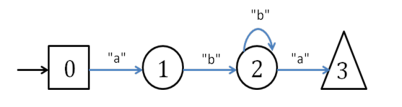
\includegraphics[width=.6\textwidth]{./images/TD1_1.png}
\end{figure}
\vspace{-0.5cm}

\begin{enumerate}
 \item Quel est l'alphabet de cet automate ?
 \item Quels sont les états de cet automate ? L'état initial et l'état final ?
 \item Quel mot cet automate permet-il de reconnaître ?
 \item L'automate permet-il de reconnaître un autre mot ? Pourquoi ?
\end{enumerate}
\setboolean{long}{true}   

\ifthenelse{\boolean{long}}{
%\noindent\fcolorbox{black}{orange}{
%\begin{minipage}{16cm}
\textbf{Réponses}

\begin{enumerate}
 \item "a" et "b"
 \item Il a 4 états, 0 (initial), 1, 2 et 3 (final)
 \item "abba" par exemple
 \item Oui, puisque l'on peut utiliser la transition de l'état 2 vers lui même autent de fois que l'on veut (y compris zéro). On peut former tous les mots de la forme "abb*a". On a au moins un "b", et le "*" signifie que l'on peut y ajouter un nombre de "b" supérieur ou égal à zéro. Mais ce n'est pas "ab*a" puisqu'on a au moins un "b". Au contraire, l'automate ci-dessous, qui n'autorise pas de choix dans les transitions ne reconnaîtra que "abba" : 
\end{enumerate}
\begin{figure}[h]
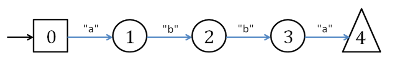
\includegraphics[width=.6\textwidth]{images/TD1_0.png}
\caption{Automate reconnaissant uniquement "abba"\label{automate-lineaire}}
\end{figure}
\vspace{-0.5cm}
%\end{minipage}
%}
\newpage
}{ ~}

\exer

\vspace{-0.5cm}
\begin{figure}[h]
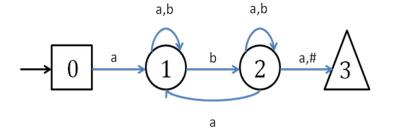
\includegraphics[width=.6\textwidth]{images/TD1_2.png}
\end{figure}

\begin{enumerate}
 \item Cet automate accepte-t-il le même mot que l'automate de l'exercice 1 ?
 \item Quelle est alors la différence ?
 \item Pouvez-vous lister les mots acceptés ?
\end{enumerate}

\ifthenelse{\boolean{long}}{
%\noindent\fcolorbox{black}{orange}{
%\begin{minipage}{16cm}
\textbf{Réponses}

\begin{enumerate}
 \item Oui, il pourra reconnaître n'importe lequel des mots reconnus par l'automate de l'exercice 1
 \item La différence, c'est qu'il en reconnaît d'autres, par exemple je peux boucler sur l'état 1 et former des mots commençant par "aa"
 \item On ne peut pas lister les mots puisque le nombre de boucle n'est pas contraint, le nombre de mots reconnaissable est infini. Tous les mots commençant par "a" puis "[ab]*b" ensuite il est possible de boucler sur l'état 2 avec "[ab]*" ou de repartir vers l'état 1 avec un "a" et de repartir sur la séquence "[ab]*b[ab*]". A l'état 2 on peut aussi choisir la transition vers l'état final avec "a" ou "\#".
\end{enumerate}
%\end{minipage}
%}

}{ ~}
\exer
\vspace{-0.3cm}
\begin{enumerate}
  \item  Dessinez un automate ne permettant d'accepter que le mot "amasser".

\ifthenelse{\boolean{long}}{\textcolor{red}{L'automate sera purement linéaire  puisque l'on ne peut s'autoriser de boucle sur le "s", il en faut 2, pas plus pas moins.}}{~}%%(comme l'automate de la figure\ref{automate-lineaire}
  \item  Listez les états et l'alphabet de votre automate.
\ifthenelse{\boolean{long}}{\textcolor{red}{ 8 états (de 0 l'état initial à 8 l'état final) et un alphabet de 5 éléments : {"a", "m", "s", "e", "r"}}}{~}
  \item  Modifiez l'automate que vous venez de dessiner afin qu'il accepte le mot "amasser", mais aussi le mot "amas".
\ifthenelse{\boolean{long}}{\textcolor{red}{Il suffit de transformer l'état 4 (le premier "s") en état final}}{~}
\end{enumerate}

\exer

Le vocabulaire de l'automate ci-dessous est composé de D, N, V, et P. Avec : D = Déterminant ; N = Nom ; V = Verbe ; P = Ponctuation

\begin{figure}[h]
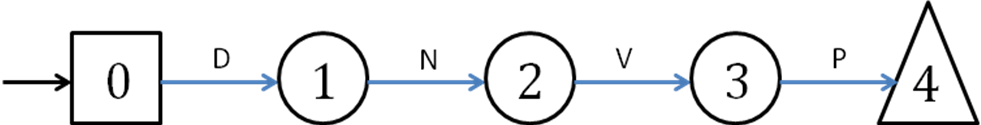
\includegraphics[width=.6\textwidth]{images/TD1_3.png}
\end{figure}


  Cet automate peut décrire la structure grammaticale d'une phrase.
 Parmi ces phrases, lesquelles sont des mots du langage décrits par l'automate ?
\begin{multicols}{2}
\begin{enumerate}
   \item La fille court. 
\ifthenelse{\boolean{long}}{\textcolor{red}{OUI, on a bien une séquence Déterminant, Nom, Verbe, Ponctuation}}{~}
   \item Le soleil brille. 
\ifthenelse{\boolean{long}}{\textcolor{red}{idem}}{~}
   \item Les pierres tombent
\ifthenelse{\boolean{long}}{\textcolor{red}{Il manque la ponctuation}}{~}
   \item Il fait chaud. 
\ifthenelse{\boolean{long}}{\textcolor{red}{Echoue sur l'item 1}}{~}
   \item Nous mangeons au restaurant.
\ifthenelse{\boolean{long}}{\textcolor{red}{Echoue sur l'item 1}}{~}
   \item Le poisson est rudement bon.
\ifthenelse{\boolean{long}}{\textcolor{red}{La séquence "rudement bon" (Adverbe Adjectif) n'est pas reconnue par l'automate}}{~}
\end{enumerate}
\end{multicols}



\exer

\begin{figure}[h]
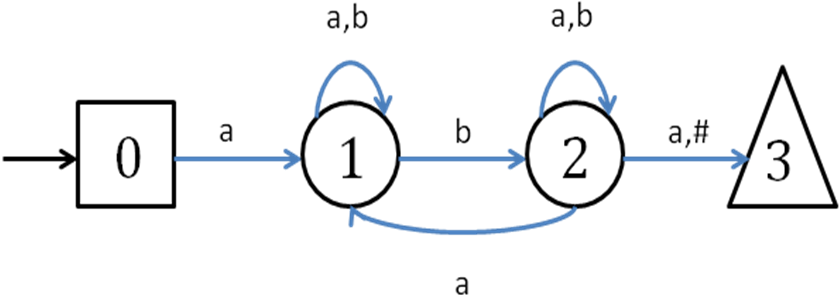
\includegraphics[width=.6\textwidth]{images/TD1_5.png}
\caption{Automate \textsc{toto}}
\end{figure}

 Dans le tableau \ref{exer5} vous trouverez le détail des règles de transition de l'automate \textsc{toto}. Par exemple la première ligne que dans l'état 0, je peux suivre la transition "a" qui m'amène dans l'état 1. Comme c'est la seule ligne où 0 est l'état courant, cela signifie que je n'ai qu'un possibilité de transition à partir de cet état. Au contraire, les lignes 2 à 4 de ce même tableau montrent qu'à partir de l'état 1, j'ai plusieurs choix.
\begin{small}
\begin{table}[h]
\centering
\begin{subtable}{.6\textwidth}

\begin{tabular}{|c|c|c|}
\hline
État courant&valeur&\'Etat de sortie\\
\hline
0	&a	&1\\
\hline
1	&a	&1\\
\hline
1	&b	&1\\
\hline
1	&b	&2\\
\hline
2	&a	&2\\
\hline
2	&b	&2\\
\hline
2	&a	&1\\
\hline
2	&a	&3\\
\hline
2	&\#	&3\\
\hline
\end{tabular}
\caption{Règles de transition de \textsc{toto} \label{exer5}}
\end{subtable}%
\begin{subtable}{.3\textwidth}
\centering
\begin{tabular}{|r|c|c|c|}
\hline
~		&a	&b	&\#\\
\hline
$\rightarrow$ 0	&1	&~	&~\\
\hline
1		&1	&1, 2	&~\\
\hline
2		&1, 2, 3&2	&3\\
\hline
* 3		&	&	&\\
\hline
\end{tabular}
\caption{Table de transitions de \textsc{toto} \label{exer5b}}
\end{subtable}
%\caption{Description de l'automate \textsc{toto}}
\end{table}
\end{small}

 Ces règles de transition peuvent être réduites dans une table de transitions. Les colonnes représentent les symboles de l'alphabet utilisé, et les lignes correspondent aux états. La table de transition est suffisante pour décrire complètement l'automate. C'est une sorte de résumé (cf . tableau  \ref{exer5b})


\begin{enumerate}
  \item  Écrivez la table de transition de l'automate présenté dans l'exercice 2
  \item  Dessinez l'automate correspondant à la table de transition du tableau \ref{exer5c} :
\end{enumerate}

\begin{center}
\begin{table}[h]
\begin{tabular}{|r|c|c|}
\hline
%\rowstyle{\bfseries}
~		&a	&b	\\
\hline
$\rightarrow$ 1	&1	&2	\\
\hline
2		&1	&1, 2	\\
\hline
\end{tabular}
\caption{Table de transitions \label{exer5c}}
\end{table}
\end{center}

\exer


\vspace{-0.5cm}
\begin{figure}[h]
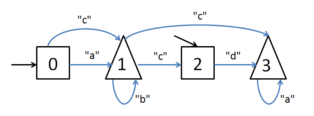
\includegraphics[width=.6\textwidth]{images/TD1_7b.png}
\end{figure}
\begin{enumerate}
  \item  Listez les états de cet automate,
et indiquez les états finaux et
initiaux.
  \item  Listez l'alphabet.
  \item  Indiquez la succession d’états permettant d’accepter chacun des mots du tableau ci-après :

\end{enumerate}

\begin{center}
\begin{table}[h]
\begin{tabular}{|c|p{6cm}||c|p{6cm}|}
\hline
%\rowstyle{\bfseries}
Mot		&Parcours?	&Mot	&Parcours?\\
\hline
a		&		&cc	&		\\
\hline
aacd		&		&d	&		\\
\hline
aaac		&		&bcd	&		\\
\hline
acdaa		&		&dd	&		\\
\hline
ac		&		&b	&		\\
\hline
abbb		&		&ccaaaaa&		\\
\hline
\end{tabular}
\end{table}
\end{center}
\exer
\begin{enumerate}
  \item  Représentez l'automate susceptible de reconnaître une structure de type sujet--verbe--complément (sans entrer dans le détail), en ayant la possibilité d'y intercaler
un – et un seul – adverbe. Exemple de mots acceptés : "Il aime beaucoup le travail."
et "Ce garçon pense souvent à toi."
  \item  Représentez l'automate acceptant uniquement les mots "machin", "machine",
"machiner", "machinerie". Optimisez l'automate au maximum, en repérant les
racines communes de ces mots.
\end{enumerate}

\exer
Représentez sous forme d'automate la navigation dans les menus d'une application de jeu,
en suivant ces consignes:
% L'écran d'introduction demande d'abord si l'utilisateur veut jouer : si oui, alors on
%montre le MENU, si non, on affiche le message de confirmation pour quitter le jeu.
% Dans le MENU, on propose à l'utilisateur ces choix :
\begin{itemize}
  \item  de créer un nouveau personnage, qui amène à l'écran de création de
personnage,
  \item  de configurer le jeu, qui amène au panneau de configuration,
  \item  d'aller vers l'éditeur de parties, qui charge cet éditeur,
  \item  de débuter le jeu en chargeant une partie existante.
\end{itemize}
% Pour les quatre choix précédents, indiquez dans votre automate qu'il est possible de
%revenir au MENU.
% Depuis l'écran de création de personnage, il est également possible de lancer le jeu.

\noindent\fcolorbox{red}{lightgray}{
\begin{minipage}{12cm}
\subsection*{Ouverture}
Des vidéos d'applications (expérimentales ou pratiques) mettant en œuvre des machines de Turing ou des Automates à Etats Finis.
\begin{itemize}
  \item La Machine de Turing réalisée Doc. retraçant l'implantation d'un
calculateur par des étudiants de l'ENS Lyon avec des Legos : 
\begin{itemize}
  \item \url{https://tinyurl.com/turing-realisee}
\end{itemize}
%ou "Machine de Turing réalisée" sur Dailymotion.
  \item Machine de Turing sur Minecraft Utilisation des mécanismes logiques du jeu Minecraft pour implanter un calculateur en 3D. Démonstrations sur quelques calculs simples... avec un mécanisme très complexe:
\begin{itemize}
  \item \url{https://www.youtube.com/watch?v=1X21HQphy6I}
\end{itemize}
%ou "Machine de Turing sur Minecraft" sur Youtube.
%  \item FSM to control your game's flow. Tutoriel vidéo pour l'implantation d'automates à états finis (Finite State Machines, FSM) pour gérer la navigation dans une application :
%\begin{itemize}
%  \item \url{http://gotoandlearn.com/play.php?id=154}
%\end{itemize}
\end{itemize}
\end{minipage}
}


\end{document}
